\documentclass[12pt]{article}

\usepackage[onlytext]{MinionPro}
\usepackage{microtype}

\setlength{\parindent}{0in}                                                     % No indentation for every paragraph

\usepackage[left=3cm, right=3cm]{geometry}		                                % Margins left and right
\usepackage{hyperref}                                                           % Clickable table of contents in PDFs
\usepackage{datetime}                                                           % Currenttime

\usepackage{physics}
\usepackage{listings}                                                           % Code inclusion
\usepackage{color}

\usepackage{float}
\usepackage{graphicx}

\definecolor{codegreen}{rgb}{0,0.6,0}
\definecolor{codegray}{rgb}{0.5,0.5,0.5}
\definecolor{codepurple}{rgb}{0.58,0,0.82}
\definecolor{backcolour}{rgb}{0.95,0.95,0.92}

\lstdefinestyle{mystyle}{
    backgroundcolor=\color{backcolour},
    commentstyle=\color{codegreen},
    keywordstyle=\color{magenta},
    numberstyle=\tiny\color{codegray},
    stringstyle=\color{codepurple},
    basicstyle=\ttfamily,
    breakatwhitespace=false,
    breaklines=true,
    captionpos=b,
    keepspaces=true,
    numbers=left,
    numbersep=5pt,
    showspaces=false,
    showstringspaces=false,
    showtabs=false,
    tabsize=2
}

\lstset{style=mystyle}

\lstset{ %
    language=C++,
    style=mystyle
}

\title{The libint-eigen interface}
\author{Laurent Lemmens}
\date{\today \hspace{6pt} \currenttime}

\begin{document}

\maketitle

\begin{center}
\line(1,0){250}
\end{center}

\tableofcontents
\newpage



\section{Terminology}
    In the LibInt2 basis set context, there is some terminology that should be cleared up. A (non-normalized) Cartesian \textit{primitive Gaussian}, centered on $\vb{R}(X,Y,Z)$, is a function of the following form:
    \begin{equation}
        \varphi(\vb{r}; \zeta, \vb{n}, \vb{R}) = (x - X)^{n_x} (y - Y)^{n_y} (z - Z)^{n_z} \exp(-\zeta |\vb{r}-\vb{R}|^2) \thinspace ,
    \end{equation}
    in which $\vb{n}(n_x, n_y, n_z)$ are called the cartesian angular momenta of the primitive. The sum
    \begin{equation}
        l = n_x + n_y + n_z
    \end{equation}
    of the angular momenta, called the \textit{angular momentum} of a primitive, determines its the type: $l=0$ refers to an $s$-type, $l=1$ to a $p$-type, etc. In general, there are\footnote{Number of ways to divide $l$ balls in $3$ urns: \href{https://en.wikipedia.org/wiki/Combination\#Number\_of\_combinations\_with\_repetition}{number of combinations with repetition}}
    \begin{equation}
        \binom{l + 3 - 1}{3 - 1} = \frac{(l+1)(l+2)}{2}
    \end{equation}
    primitives corresponding to a given angular momentum $l$. For example, the following primitives all belong to the case $l=1$ (i.e. for $p$-type orbitals):
    \begin{equation}
        \varphi_{p_x}(\zeta) \qquad \varphi_{p_y}(\zeta) \qquad \varphi_{p_z}(\zeta) \thinspace ,
    \end{equation}
    where we have introduced a short-hand notation for primitives: the exponents are given as arguments, the type is given as subscript, and the center is omitted (and to be deduced from context). For clarity:
    \begin{equation}
        \varphi_{p_x}(\zeta) \equiv \varphi(\vb{r}; \zeta, \vb{n}=(1,0,0), \vb{R}) = (x - X) \exp(-\zeta |\vb{r}-\vb{R}|^2) \thinspace .
    \end{equation}

    In the following, we will refer to a set of Gaussian primitives with the same angular momentum $l$ that share the same center as a \textit{shell}. \\

    Often, a predetermined/fixed linear combination (also known as a \textit{contraction}) of primitives is taken, leading to a \textit{contracted GTO} (CGTO):
    \begin{equation}
        d_1 \varphi_s(\zeta_1) + d_2 \varphi_s(\zeta_2) \thinspace ,
    \end{equation}
    in which the \textit{contraction coefficients} $d$ have to be specified. CGTOs are the functions that are used as \textit{basis functions} (\textit{atomic orbitals}: AOs). Note that a single primitive can also be used as a basis function, in which case the linear combination is just one times that primitive. A graphical explanation of the different concepts of primitives, CGTOs, basis functions and shells is given in Figure \ref{fig:basis}\\

    \textit{Molecular orbitals} (MOs) are then written as a linear combination of AOs (which are CGTOs), which in turn serve as a one-electron basis to antisymmetrize into the many-electron basis of the \textit{Slater determinants} (SDs). \cite{jensen2007} \\

    Internally, LibInt2 stores (normalized) contraction coefficients and exponents in \lstinline{libint2::Shell} objects.

    \begin{figure}[H]
        \centering
        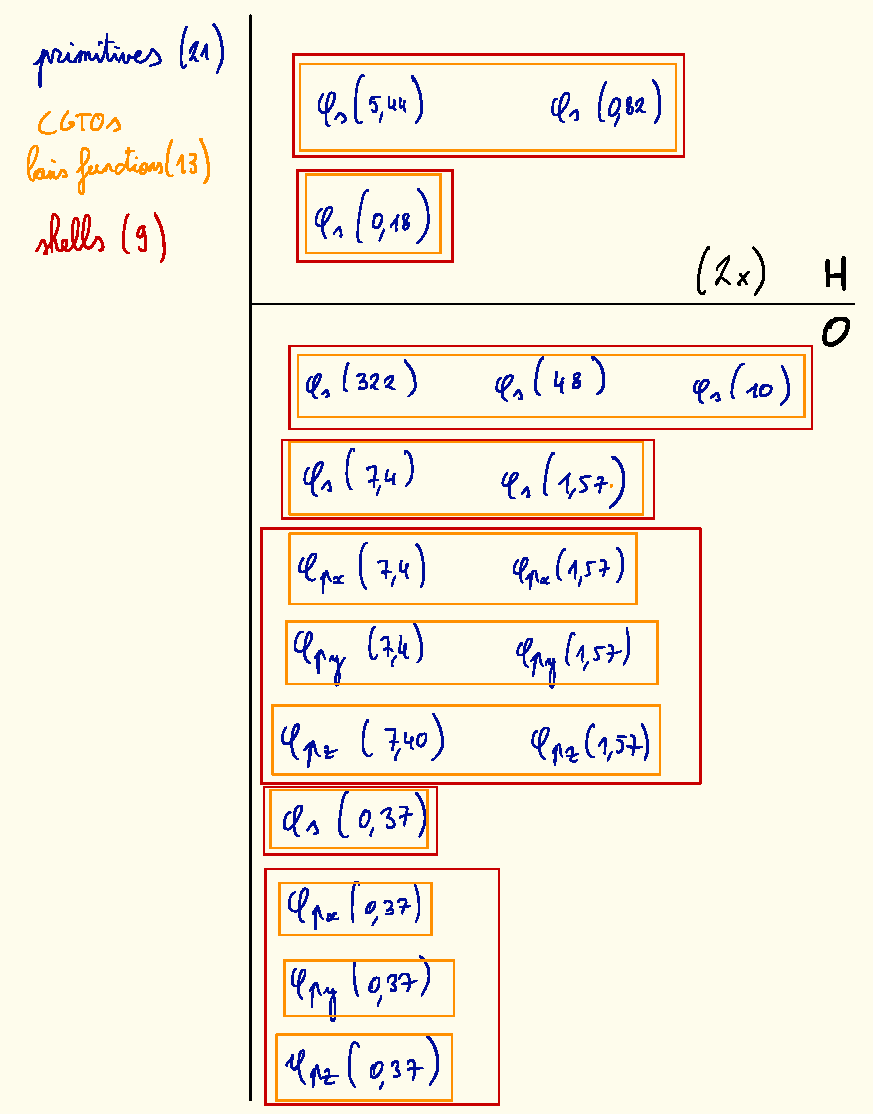
\includegraphics[scale=0.65]{figures/H2O_3-21g.pdf}
        \caption{Explanation of the concepts of primitives, CGTOs (basis functions) and shells for water @ 3-21G. $\varphi$ denotes a Gaussian primitive, its argument being the value of the exponent and its subscript specifying its angular momentum.}
        \label{fig:basis}
    \end{figure}


\section{Are the basis functions (CGTOs) normalized?}

    When constructing a \lstinline{libint2::BasisSet} object as in say

\begin{lstlisting}
libint2::BasisSet obs ("STO-3G", atoms);
\end{lstlisting}

    the corresponding file \lstinline{sto-3g.g94} is read (which is located at your \lstinline{LIBINT_DATA_PATH} environment variable), in which LibInt2 finds the exponents and contraction coefficients for the given basis for a given element. \\

    In \lstinline{libint2/basis.h}, we can see the following code (edited for brevity):

\begin{lstlisting}
static ... read_g94_basis_library(...){
    ...
    ref_shells[Z].push_back(
        libint2::Shell{...}
        )
    ...
}
\end{lstlisting}

    which calls a specific constructor of \lstinline{libint2::Shell}:

\begin{lstlisting}
Shell(...) {
    // embed normalization factors into contraction coefficients
    renorm();
}
\end{lstlisting}

    that makes sure that the CGTO is normalized by including the normalization factor in the contraction coefficients. So, \textbf{yes}, LibInt2 internally works with normalized basis functions.



% % % REFERENCES % % %

\newpage

\bibliographystyle{unsrt}                                                       % Bibliography in chronological order
\bibliography{/Users/laurentlemmens/Documents/Archief/Bibliotheek/research_bib.bib}

\end{document}
